\documentclass[12pt,a4paper]{article}
\usepackage{algorithm}
\usepackage{algpseudocode}
\usepackage{listings}
\usepackage{marvosym}
\usepackage{wasysym}
\usepackage{marvosym}
\usepackage{xcolor}
\usepackage{graphicx}
\usepackage{tikz}
\usepackage{tikz-uml}
\usetikzlibrary{positioning,shapes,arrows}
\usetikzlibrary{calc,shapes.multipart,chains,automata,positioning,shapes,arrows,backgrounds,fit}
\usetikzlibrary{matrix,backgrounds}

\author{Sujit Chakrabarti}
\title{ArrayLists and Linked Lists}
\date{}

\begin{document}
\definecolor{lightblue}{rgb}{0.8,0.93,1.0} % color values Red, Green, Blue
\definecolor{Blue}{rgb}{0,0,1.0} % color values Red, Green, Blue
\definecolor{Red}{rgb}{1,0,0} % color values Red, Green, Blue
\definecolor{Purple}{rgb}{0.5,0,0.5}
\definecolor{Pink}{rgb}{0.7,0,0.2}

\newcommand{\highlight}[1]{{\color{Red}(#1)}}
\newcommand{\comment}[1]{{\color{Blue}#1}}

\lstset{
	language = Java,
	basicstyle = \ttfamily\scriptsize,
	stringstyle = \ttfamily\scriptsize,
	keywordstyle=\color{black}\scriptsize,
	identifierstyle=\color{black}\scriptsize,
	frameround=tttt,
	numbers=none,
	showstringspaces=false
}

\maketitle

\section{Why Collections?}
There are situations in programming where the data you are interested in represents collection of smaller things. Consider the institute information management system. We create one object of the \lstinline@Student@ class corresponding to each student. In order to implement any functionality that requires the entire collection of students to be available at once, we need to keep these objects in a single place. One example is \lstinline@printStudentList@ method which prints all the students. Another example could be \lstinline@search@ method.

From what have learnt so far, we could use arrays for this purpose as shown in fig.~\ref{f:array}.

\begin{figure}[H]
	\lstinputlisting{code/WithArray.java}
\caption{Representing List of Students using Java arrays}
\label{f:array}
\end{figure}


Arrays have a few advantages, namely they are simple to create and it's easy to access elements within an array. However, there's a big disadvantage. Once an array object is created, you can't add anything to it, nor can you delete any element from it. And this is a serious problem for the Institute Information Management System we have been building. For example, if you wish to enrol a student, you would like to add this student into the array. But Java arrays don't allow you to do this: once you have created an array, you are allowed to modify its elements, but you can't expand or shrink it.

Can we have an array which allows us the functionality of arrays along with the flexibility to expand or shrink it as required. Yes, we can do this using Java lists.

In this section, we will learn about two types of lists: \lstinline@ArrayList@, and \lstinline|LinkedList|. Apart from learning how to use them, we also discuss how one can often be used in place of the other rather seamlessly. We also discuss the various trade-offs between the two types of lists.

In summary:
\begin{enumerate}
	\item  This module is an introduction to the use of data-structures as a fundamental mechanism for implementing robust and efficient programs.
	\item We get to discuss -- although briefly and indirectly -- how such data-structures are typically implemented in an object-oriented language like Java.
	\item Finally, this segment is a gentle primer to the much larger and very important topic of data-structures and algorithms, for which we have reserved an entire module of the course.
	
\end{enumerate}

\begin{figure}[H]
	\lstinputlisting{code/WithArrayList.java}
	\caption{Representing List of Students using Java \lstinline|ArrayList| (code/WithArrayList.java)}
	\label{f:al}
\end{figure}

One possible way of storing the list of students is shown in fig.~\ref{f:al}. And one of the advantages of this type is immediately evident here: Note that we are adding elements to this list one after another. This is equivalent to being able to enrol students as and when we wish. As we will show shortly, it's equally easy to remove a student from the rolls.

\section{Generics}
One of the issues with the code in fig.~\ref{f:al} is about \emph{type safety}. A type-safe program is one which doesn't or can't encounter a runtime type error. The \lstinline@ArrayList@ we have used can have objects of any class which is a sub-type of \lstinline@Object@. As a result, we are forced to use type-casting in printStudentList method to obtain a \lstinline@Student@ from an \lstinline@Object@. This is essential so that we can access the \lstinline@getDetails@ method of the \lstinline@Student@ class. Such type-casting, although unavoidable in certain rare circumstances, is an inherently unsafe thing to do as they may lead to runtime type errors.

To understand this, consider the line which has been commented out in the \lstinline@main@ method:
\begin{lstlisting}
studentList.add(new String("Hari"));
\end{lstlisting}

If this code is uncommented, this will add a string to the \lstinline@studentList@ in which all other elements happen to be of \lstinline@Student@ type. The result of running this code will as follows:
\begin{lstlisting}
name = Sujit
roll number = 1

name = Siddharth
roll number = 2

name = Karanpreet
roll number = 3

Exception in thread "main" java.lang.ClassCastException:
  java.lang.String cannot be cast to Student
at WithArrayList.printStudentList(WithArrayList.java:16)
at WithArrayList.main(WithArrayList.java:11)
\end{lstlisting}

This output is not surprising, and demonstrates a vulnerability of the given code which comes inherently with use of \lstinline@ArrayList@ of \lstinline@Object@s. The solution to this problem lies in being able to make the type of the \lstinline@ArrayList@ more specific: to be able to say that it should an \lstinline@ArrayList@ that is allow to have elements of \lstinline@Student@ type and none else. Turns out, it's possible to do this, using Java generics. The modified code is shown in fig.~\ref{f:alg}.

\begin{figure}
	\lstinputlisting{code/WithArrayListGeneric.java}
\caption{ArrayList using Java Generics (\texttt{code/WithArrayListGeneric.java})}
\label{f:alg}
\end{figure}

Note the following:
\begin{enumerate}
	\item The typecasting needed in \lstinline@printStudentList@ method of fig.~\ref{f:al} is no more needed.
	\item The commented line in \lstinline@main@ method, if uncommented, would lead to a compile error (instead of a runtime error as in fig.~\ref{f:al}). This is definitely better, as Java's type-system is helping us detect a potential runtime type error at compile time.
\end{enumerate}
Also note that Java arrays were already type safe as we have used them in our examples. By starting to use \lstinline@ArrayList@ in a non-generic way, we had lost out on that type-safety. However, by bringing in generics, we have got it back now. All container classes shipped with Java are implemented using generics. Using them is almost exactly the same as how you use \lstinline@ArrayList@ and \lstinline@LinkedList@. We have briefly explained how to \emph{use} these classes. How Java generics is used to implement these -- and other similar -- classes is a topic beyond the scope of this discussion.

\section{Linked List}
All that we have done in the last two pieces of code that we developed, can also be done pretty much exactly the same way with another kind of list, called the \emph{linked list}. \lstinline@LinkedList@ class of \lstinline@java.util@ package gives us an implementation of this data-structure. The above sets of code have been developed using \lstinline@LinkedList@ in fig.~\ref{f:ll} (type unsafe) and fig.~\ref{f:llg} (type safe using generics).

\begin{figure}
	\lstinputlisting{code/WithLinkedList.java}
	\caption{\lstinline@LinkedList@ (\texttt{code/WithLinkedList.java})}
	\label{f:ll}
\end{figure}

\begin{figure}
	\lstinputlisting{code/WithLinkedListGeneric.java}
	\caption{\lstinline@LinkedList@ using Java Generics (\texttt{code/WithLinkedListGeneric.java})}
	\label{f:llg}
\end{figure}

\section{\lstinline@List@ and Polymorphism}
The reason why we have almost identical set of features in \lstinline@LinkedList@ class and \lstinline@ArrayList@ class is because these features are really those of the \lstinline@List@ class (again in \lstinline@java.util@ package) of which \lstinline@LinkedList@ class and \lstinline@ArrayList@ class are sub-classes. The internal implementation of \lstinline@List@ class of which \lstinline@LinkedList@ class are different which leads to different runtime performance characteristics for these two classes (more about this in sec. ~\ref{s:alvsll}). However, both of them have nearly identical, governed by the interface of the \lstinline@List@ class. Let's see an example of how the \lstinline@List@ class, along with some clever use of polymorphism, can be used to implement some nice and reusable piece of code.

\begin{figure}
	\lstinputlisting{code/ListPolymorphism.java}
	\caption{\lstinline@List@ and Polymorphism (\texttt{code/ListPolymorphism.java})}
	\label{f:lp}
\end{figure}

Fig.~\ref{f:lp} shows a piece of code where we have used both \lstinline@ArrayList@ and \lstinline@LinkedList@ class. Both \lstinline@studentList1@ and \lstinline@studentList2@ are \lstinline@List<String>@ type. However, they are being initialised with an object of the class \lstinline@ArrayList<String>@ and \lstinline@LinkedList<String>@ respectively. Both these \lstinline@List@s are passed in turn to the \lstinline@printStudents@ method which takes a parameter of the type \lstinline@List<String>@ type.

The output of running the code is as shown below:
\begin{lstlisting}
Printing student list ...
Student number 0 : Tricha
Student number 1 : Murali
Student number 2 : Sujit
Printing student list ...
Student number 0 : Siddharth
Student number 1 : Karanpreet
\end{lstlisting}


\section{List Iterators}


\section{Choosing between the Various List Implementations} \label{s:alvsll}
As we have seen through the various examples, what you can do with \lstinline@ArrayList@ is pretty much the same as what you can accomplish by using \lstinline@LinkedList@. You may wonder, why then, makers of Java language have provided two different \lstinline@List@s when their capabilities are so similar. The answer lies, not in functionality, but in performance.

Let's conduct a few experiments to understand this point.

In all these experiments, we create two lists \lstinline@list1@ and \lstinline@list2@, each with a around a lakh integers. One is an \lstinline@ArrayList@ while \lstinline@list2@ is a \lstinline@Linkedlist@. We then perform the same operation on both the lists, and estimate how much time it took to perform the operation in each case. Further, you will notice that we perform the operation a large number of times. That's because we wish to make the numbers significant enough to bring out the performance differences clearly. Further, doing the same thing a large number of times also flushes out any random error in the values.

\subsection{Getting by Index}
\begin{figure}
	\lstinputlisting{code/LargeListGet.java}
	\caption{\lstinline@get@ting elements from anywhere (\texttt{code/LargeListGet.java})}
	\label{f:lg}
\end{figure}

In this experiment (see fig.~\ref{f:lg}), we perform the \lstinline@get@ operation on the large element of the long lists.
We get the following output:
\begin{lstlisting}
array value = 49999
ArrayList took 291772 ns.
array value = 49999
Linked List took 610700 ns.
ArrayList faster by  318928 ns!
\end{lstlisting}

We observe that \lstinline@ArrayList@ is significantly faster. Let me tell you that this value is not precise, since it includes the time taken by many other thinks (e.g. iterating through the loop etc.). Also, there are external factors associated with the computer itself (e.g. multiprocessing, cache-misses and page faults etc.)which have an influence on the exact amount of time needed to perform the task. However, this still give a fair estimate about which of the two elements is faster. So, it can be inferred that:

\begin{quote}
	\lstinline|ArrayList|s are faster than \lstinline|LinkedList|s when it comes to reading the values of elements at arbitrary positions in the list.
\end{quote}

\subsection{Adding at the End}
\begin{figure}
	\lstinputlisting{code/LargeListAddEnd.java}
	\caption{\lstinline@add@ing elements at the tail end of the list (\texttt{code/LargeListAddEnd.java})}
	\label{f:lae}
\end{figure}


\subsection{Adding Anywhere}
\begin{figure}
	\lstinputlisting{code/LargeListAdd.java}
	\caption{\lstinline@add@ing anywhere (\texttt{code/LargeListAdd.java})}
	\label{f:la}
\end{figure}

On running the code in fig.~\ref{f:la}, we get the following output:
\begin{lstlisting}
ArrayList took 1610172712 ns.
LinkedList took 4834461 ns.
Linked Lists faster by a factor of 333!
\end{lstlisting}

We see that linked lists are faster, not by a smaller factor, several hundred times. If we try removing elements from somewhere in the beginning of the list, you would see similar results.

The inference from this experiment is:

\begin{quote}
	\lstinline|LinkedList|s are significantly faster when elements are added/removed from arbitrary positions.
\end{quote}

\subsection{Explanation}

If you are curious to know why the observations are they way they are in the experiments just shown, you would have to delve a bit into the internal details of how these \lstinline|List|s -- \lstinline|ArrayList| and \lstinline|LinkedList| -- are built and how they work.

\subsubsection{\lstinline|ArrayList|}

\begin{figure}
\begin{center}
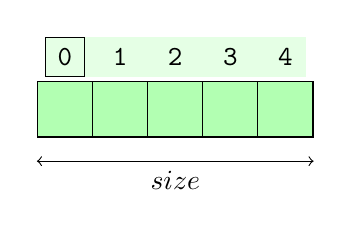
\begin{tikzpicture}[font=\ttfamily,
array/.style={matrix of nodes,nodes={draw, minimum size=7mm, fill=green!30},column sep=-\pgflinewidth, row sep=0.5mm, nodes in empty cells,
	row 1/.style={nodes={draw=none, fill=none, minimum size=5mm}},
	row 1 column 1/.style={nodes={draw}}},
carray/.style={matrix of nodes,nodes={draw, minimum size=7mm, fill=gray!30},column sep=-\pgflinewidth, row sep=0.5mm, nodes in empty cells,
	row 1/.style={nodes={draw=none, fill=none, minimum size=5mm}}}
]


\matrix[array] (array) {
	0 & 1 & 2 & 3 & 4 \\
	&   &   &   &     \\};

\begin{scope}[on background layer]


\fill[green!10] (array-1-1.north west) rectangle (array-1-5.south east);
\end{scope}

\draw[<->]([yshift=-3mm]array-2-1.south west) -- node[below] {$size$} ([yshift=-3mm]array-2-5.south east);

%
\end{tikzpicture}
\end{center}

\label{f:alsch}
\caption{ArrayList: Schematic}
\end{figure}


\begin{figure}
	\begin{center}
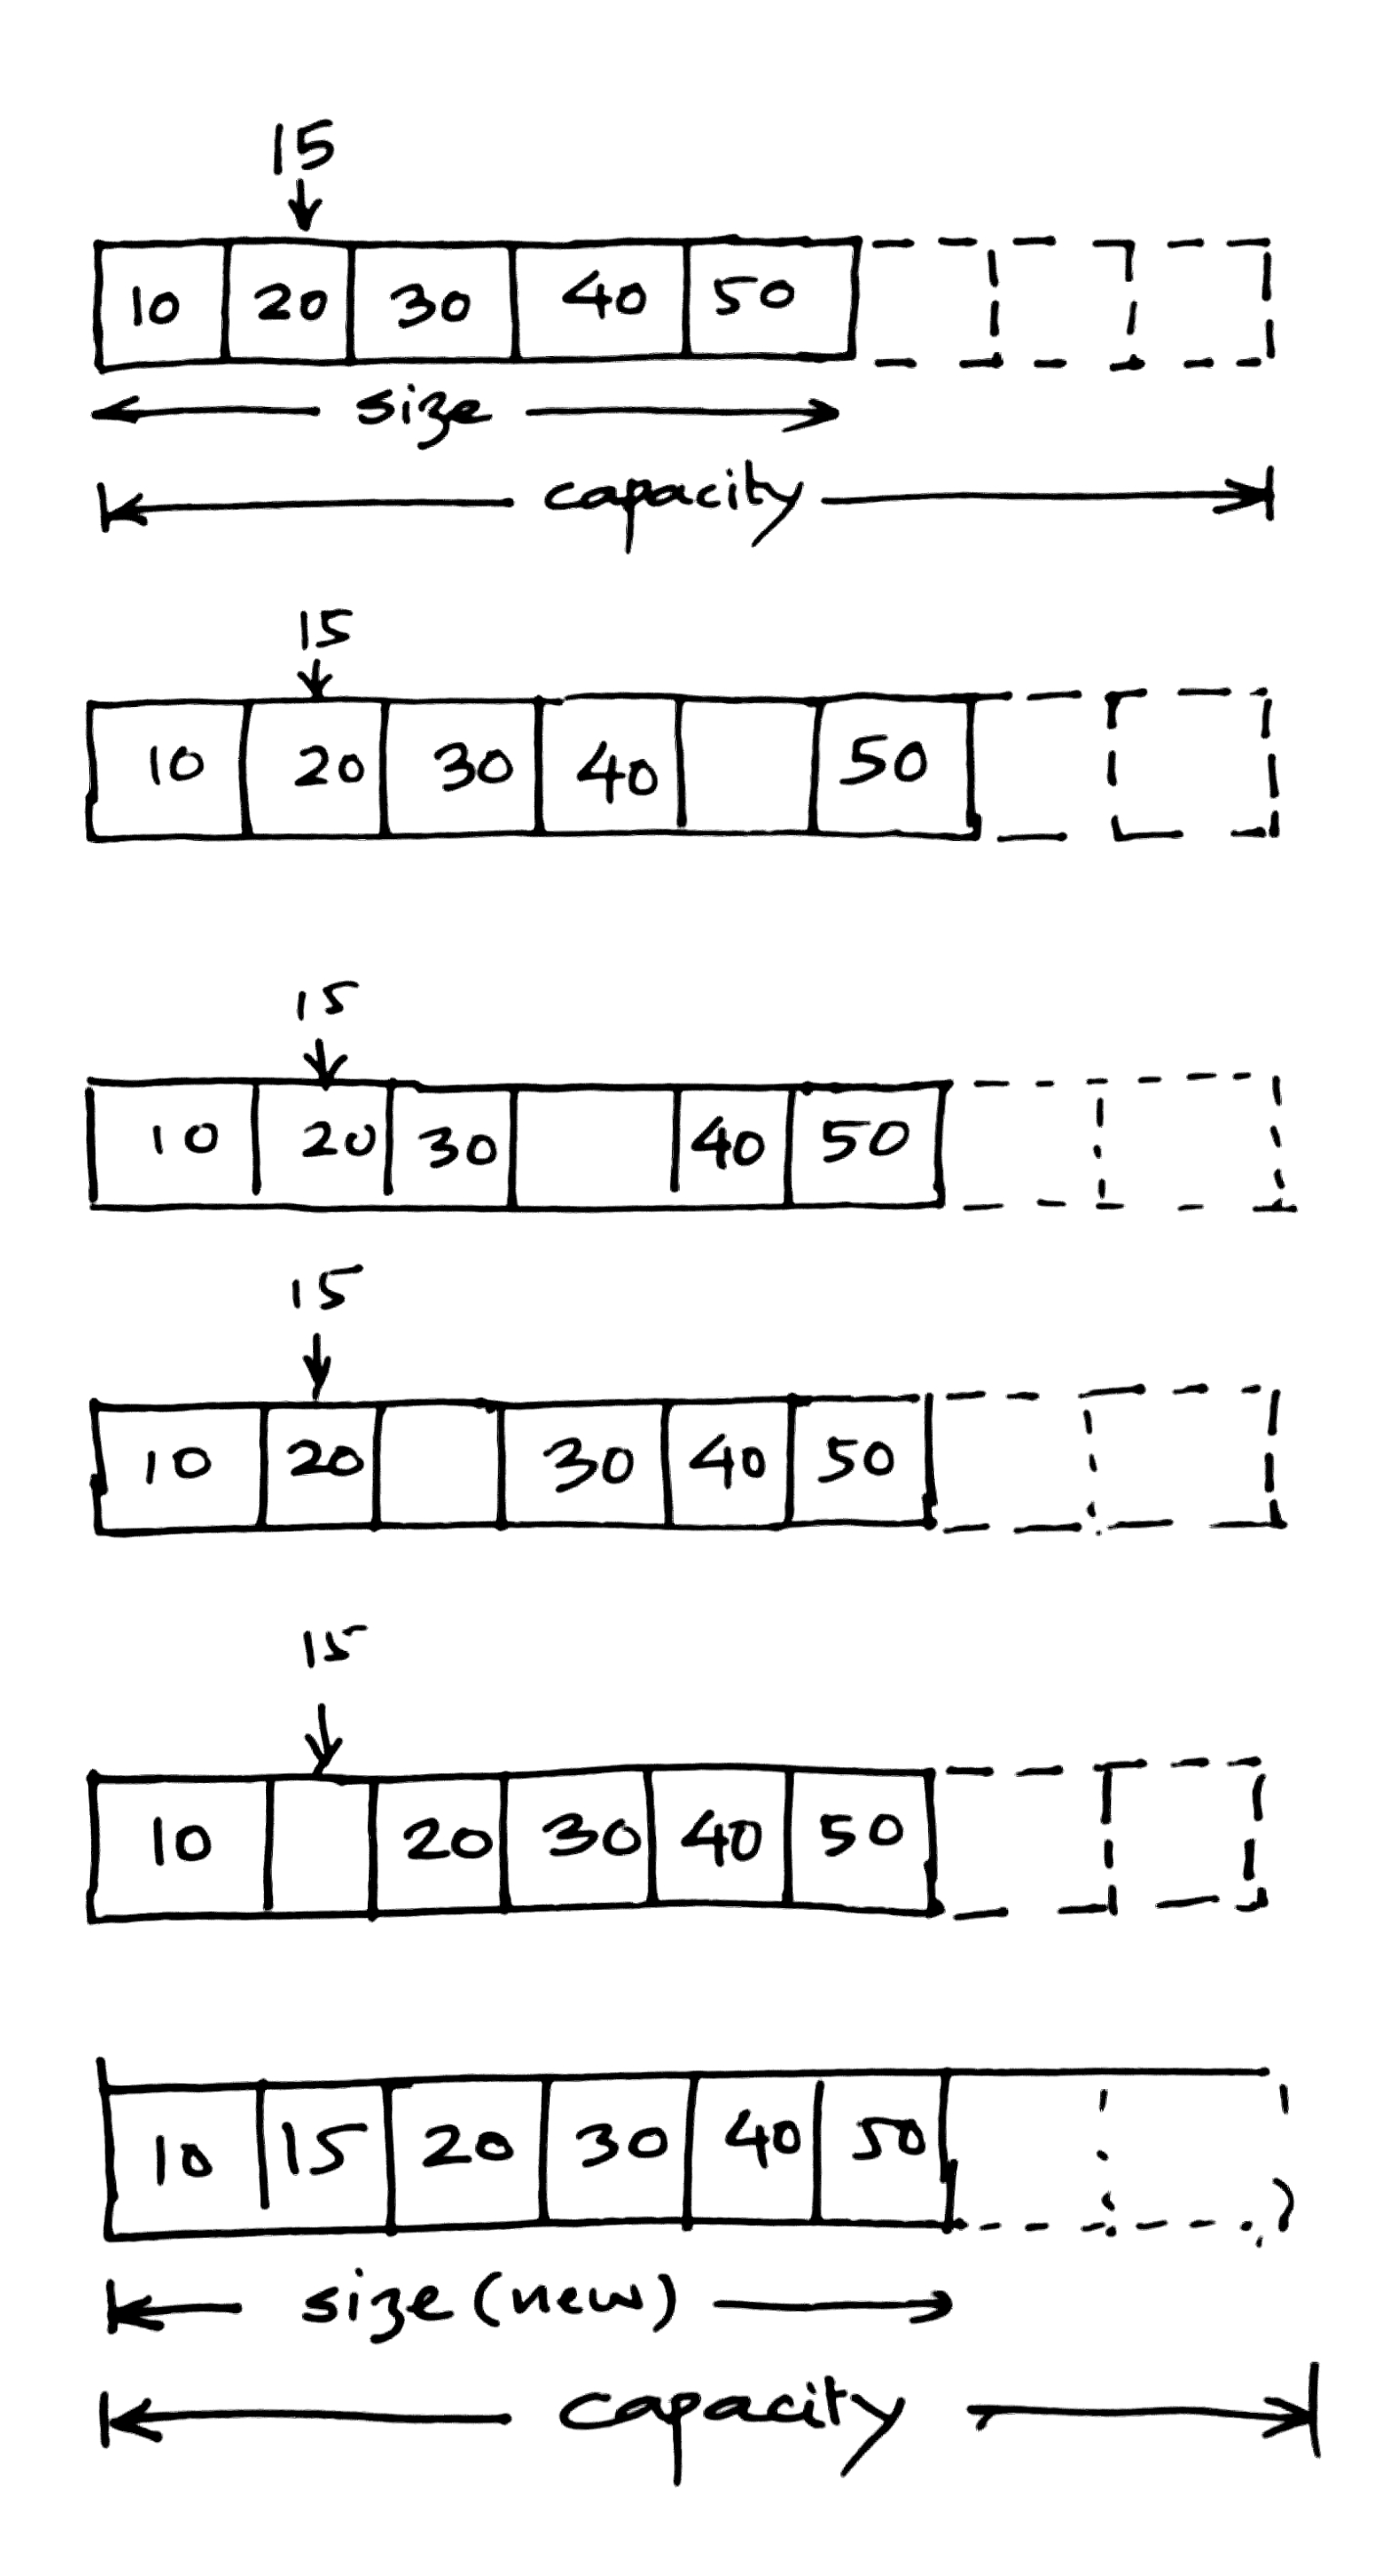
\includegraphics[width=0.7\textwidth]{array-add.jpg}
	\end{center}
	
	\label{f:aladd}
	\caption{ArrayList: Adding and element at arbitrary location}
\end{figure}

The \lstinline@ArrayList@ class uses a Java array internally. However, depending on how many elements are currently stored in the array, the capacity of the array keeps changing. Therefore, \lstinline@ArrayList@ works with two important attributes:
\begin{enumerate}
	\item size. The number of elements currently stored in the array.
	\item capacity. The actual size of the array.
\end{enumerate}

Of course, at any point the capacity must always be greater than or equal to the size. Let's call the ratio $size/capacity$ as the \emph{loading factor} $L$ of the \lstinline@ArrayList@.

To begin with, \lstinline@ArrayList@ starts off with an array $A_1$ as the internal store with some appropriate initial value of capacity. As elements get added, $A_1$ starts getting filled up. When it is close to full, indicating by $L > \tau_1$ where $tau_1$ is some threshold value, a new array $A_2$ is created with another larger capacity and all the elements in the original array are copied to the new array. This point on, the new array $A_2$ is used as the internal store; $A_1$ is discarded.

Likewise, whenever elements start getting removed, loading factor $L$ starts dropping. When $L < \tau_2$,   a new array $A_3$ is created with another smaller capacity and all the elements in the original array are copied to $A_3$. This point on, the new array $A_3$ is used as the internal store; $A_2$ is discarded.

Let's call the above events: copying $A_1$ to $A_2$, $A_2$ to $A_3$ and so on as \emph{array copy}.
\lstinline@ArrayList@ tries to keep the value of $L$ reasonably close to 1, so that the amount of wasted space is minimised (remember that at any point $capacity - size$ cells of the array are unused). On the contrary, keeping it too close to 1 would result in more frequent array copies, hitting the runtime performance of the data structure. Further, it is typically a good idea to keep $\tau_1 \neq \tau_2$ to avoid creating \emph{thrashing points}. If $\tau_1 = \tau_2$, then \lstinline@add@s and \lstinline@remove@s around these thrashing points would start getting prohibitively expensive.

Anyway, the above are some design considerations useful for implementing a data-structure like \lstinline@ArrayList@.

How does \lstinline@ArrayList@ do when \lstinline@add@s happen at the right end? Well, they are lightning fast: almost as fast as writing into a cell of an array. Similarly, for \lstinline@remove@s done at the right end. Of course, if the \lstinline@add@ causes $L$ to cross $\tau_1$ (in case of \lstinline@add@)or $\tau_2$ (in case of \lstinline@remove@), it will result in an array copy. That's expensive, but with well-chosen values of $\tau_1$ and $\tau_2$, that should be fairly rare.

But what happens when you \lstinline@add@ or \lstinline@remove@ from close to the left end of the \lstinline@ArrayList@? Well, then the things aren't as rosy as before. Let's say, you have 5 elements in your array (indices 0, 1, 2, 3 and 4), and you are \lstinline@add@ing an element at index 1. The cell at index 1 is occupied by another element. So, it must be shifted rightward (into index 2). But index 2 is also occupied by another element. So, that needs to shifted rightward to index 3. So, you get the drift, right? All the elements to the right of the index at which you wish to make the addition must be moved one place to their right. The process must begin from the right end. How many steps will the process take? In our example, 4 elements need to be shifted. In general, whenever you are \lstinline@add@ing to an \lstinline@ArrayList@ close to its left end, or to any random position for that matter, the number of elements needed to be shifted this way would be something proportional to the $size$ of the array. This is undoubtedly a fairly expensive thing to do! If your computation requirement involves lots of \lstinline@add@s and \lstinline@remove@s at arbitrary indices of the list, \lstinline@ArrayList@ would turn out to be a poor choice because of this.

\subsubsection{\lstinline|LinkedList|}

\begin{figure}
\begin{center}
	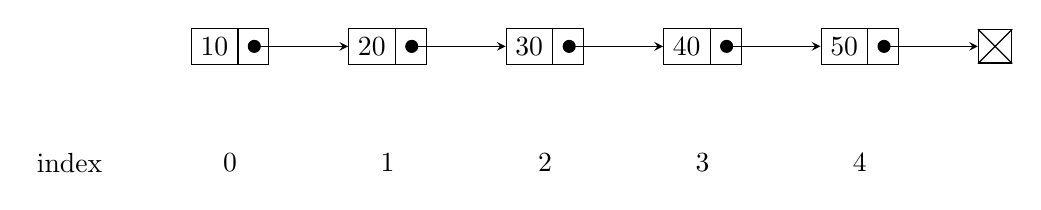
\begin{tikzpicture}[list/.style={rectangle split, rectangle split parts=2,
		draw, rectangle split horizontal}, >=stealth, start chain]
	
	\node[list,on chain] (A) {10};
	\node[list,on chain] (B) {20};
	\node[list,on chain] (C) {30};
	\node[list,on chain] (D) {40};
	\node[list,on chain] (E) {50};
	
	\node (I) [below left = of A] {index};

	\node[below = of A] (iA) {0};
	\node[below = of B] (iB) {1};
	\node[below = of C] (iC) {2};
	\node[below = of D] (iD) {3};
	\node[below = of E] (iE) {4};
	
	\node[on chain,draw,inner sep=6pt] (F) {};
	\draw (F.north east) -- (F.south west);
	\draw (F.north west) -- (F.south east);
	\draw[*->] let \p1 = (A.two), \p2 = (A.center) in (\x1,\y2) -- (B);
	\draw[*->] let \p1 = (B.two), \p2 = (B.center) in (\x1,\y2) -- (C);
	\draw[*->] let \p1 = (C.two), \p2 = (C.center) in (\x1,\y2) -- (D);
	\draw[*->] let \p1 = (D.two), \p2 = (E.center) in (\x1,\y2) -- (E);
	\draw[*->] let \p1 = (E.two), \p2 = (F.center) in (\x1,\y2) -- (F);
	\end{tikzpicture}
\end{center}	
\label{f:llsch}
\caption{Linked List: Schematic representation}

\end{figure}

\lstinline@LinkedList@ class is an implementation of the linked list data structure. This helps overcome the following drawbacks of an \lstinline@ArrayList@: 
\begin{enumerate}
	\item Array copies are expensive even though rare. They do not affect the average execution time of additions into and removals of elements from the array, the worst case time gets severely affected due to that. This may sometimely be unacceptable in certain cases, e.g. real-time systems where worst case execution times are as important as average case.
	\item Finally, additions into and removal from arbitrary positions in the list is very expensive, even in the average case, for \lstinline@ArrayList@s. This becomes the primary reason why \lstinline@LinkedList@ is sometimes the list of choice.	
\end{enumerate}

A linked list arranged its elements into dynamically created two cell nodes. The first cell of each node called the $value$ contains the value of the element; the second cell contains the reference to the next node, and hence is called the $next$ cell. The rightmost node's $next$ points to a $null$ or $nil$ address, indicating that there's nothing to the right of this.


\begin{figure}
	\begin{center}
		\resizebox{0.8\textwidth}{!}{
		\begin{tikzpicture}[list/.style={rectangle split, rectangle split parts=2,
			draw, rectangle split horizontal}, >=stealth, start chain]
		
		\node[list,on chain] (A) {10};
		\node[list,on chain] (B) {20};
		\node[list,on chain] (C) {30};
		\node[list,on chain] (D) {40};
		\node[list,on chain] (E) {50};

		\node[list] (AA) [above right = of A] {15};
		
		\node (I) [below left = of A] {index};
		
		\node[below = of A] (iA) {0};
		\node[below = of B] (iB) {1};
		\node[below = of C] (iC) {2};
		\node[below = of D] (iD) {3};
		\node[below = of E] (iE) {4};
		
		\node[on chain,draw,inner sep=6pt] (F) {};
		\draw (F.north east) -- (F.south west);
		\draw (F.north west) -- (F.south east);
		\draw[*->] let \p1 = (A.two), \p2 = (A.center) in (\x1,\y2) -- (B);
		\draw[*->] let \p1 = (B.two), \p2 = (B.center) in (\x1,\y2) -- (C);
		\draw[*->] let \p1 = (C.two), \p2 = (C.center) in (\x1,\y2) -- (D);
		\draw[*->] let \p1 = (D.two), \p2 = (E.center) in (\x1,\y2) -- (E);
		\draw[*->] let \p1 = (E.two), \p2 = (F.center) in (\x1,\y2) -- (F);
		\end{tikzpicture}
}
	\end{center}	

	\begin{center}
		\resizebox{0.8\textwidth}{!}{
			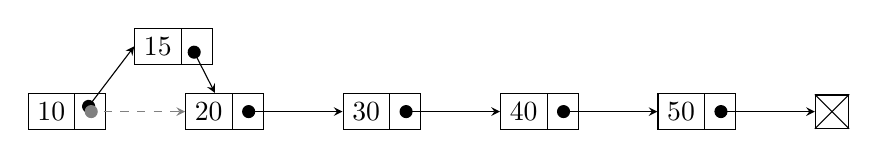
\begin{tikzpicture}[list/.style={rectangle split, rectangle split parts=2,
				draw, rectangle split horizontal}, >=stealth, start chain]
				
				\node[list,on chain] (A) {10};
				\node[list,on chain] (B) {20};
				\node[list,on chain] (C) {30};
				\node[list,on chain] (D) {40};
				\node[list,on chain] (E) {50};
				
				\node[list] (AA) [above right = 0.5cm of A] {15};
				
				
				\node[on chain,draw,inner sep=6pt] (F) {};
				\draw (F.north east) -- (F.south west);
				\draw (F.north west) -- (F.south east);
				\draw[*->] let \p1 = (A.two), \p2 = (A.center) in (\x1,\y2) -- (AA.west);
				\draw[*->, gray, dashed] let \p1 = (A.two), \p2 = (A.center) in (\x1,\y2) -- (B);
				\draw[*->] let \p1 = (AA.two), \p2 = (AA.center) in (\x1,\y2) -- (B);
				\draw[*->] let \p1 = (B.two), \p2 = (B.center) in (\x1,\y2) -- (C);
				\draw[*->] let \p1 = (C.two), \p2 = (C.center) in (\x1,\y2) -- (D);
				\draw[*->] let \p1 = (D.two), \p2 = (E.center) in (\x1,\y2) -- (E);
				\draw[*->] let \p1 = (E.two), \p2 = (F.center) in (\x1,\y2) -- (F);
				\end{tikzpicture}
				}
				\end{center}	

	\label{f:lladd}
	\caption{Linked List: Adding an element}
	
\end{figure}

How do we add to a linked list. Let's say that you again have a linked list with 5 elements, and you are adding at the index 1. 
\begin{enumerate}
	\item Firstly, a new node $N$ is created. The $value$ field of this node is the value you want to insert.
	\item Its $next$ field is made to point to the node at index 2 (note that the reference to this node is available in the $next$ cell of the node $N_1$ at index 0).
	\item Finally, the $next$ field of the node in index 0, which has been pointing to the $N_2$ (index 1 so far, and index 2 here on), will now be redirected to point to $N$.
\end{enumerate}
 
Done in 3 simple steps, regardless of where in the list we are making the addition.

Similarly, if you are removing from an arbitrary position, it's even simpler. Let's say, you wish to remove from index 1. Let's say that the nodes on indices 0, 1 and 2 are $N_0$, $N_1$ and $N_2$ respectively. All you need to do, to remove $N_0$ is to redirect the $next$ field of $N_0$ (which has been hitherto pointing to $N_1$) to point to $N_2$.

Due to the above property of constant time additions and removals, linked lists do very well in scenarios that involve repeated additions and removals at arbitrary index values in the list.

But all isn't hunky dory with \lstinline@LikedList@s either, for then, why would anyone have needed \lstinline@ArrayList@s. Consider doing a \lstinline@get@. In \lstinline@ArrayList@, it's just as far as accessing/reading an element from a Java array, irrespective of where in the list we are reading from. Unfortunately, with linked lists, it's not so easy. The only way to reach an element in a linked list is by starting with the first element, and hopping through the links one by one till we reach the desired index. Clearly, to \lstinline@get@ the element at index $n$ will need $n$ hops. And that's again expensive -- very expensive -- compared to \lstinline@get@ting from an \lstinline@ArrayList@. Hence, in scenarios which require repeated \lstinline@get@s or reads from arbitrary locations of the list, linked lists fare poorly as compared to array lists.

\subsection{Doubly Linked List}
There's an interesting quirk about the linked list implementation that we have introduced in this section. Operations done close to its left end are faster, while those done closer to its right end are slower \footnote{Please note that, for the data structure, in reality there's no left or right end. We are calling one of the ends as the left end (the first node of the list) and the other extreme as the right end simply because we have chosen to draw the linked list on paper that way.}. For example, \lstinline@l.get(0)@ (\lstinline@get@ at the extreme left or start of the list) will take a lot less time than \lstinline@l.get(l.size() - 1)@ (\lstinline@get@ done at the extreme right or far end of the list). This behaviour is assymmetric. Another example of assymmetric behaviour is in the performance of the forward and backward iterator. The forward iterator (moving from the left to the right end, or from the beginning of the list to the end of it) will perform must faster than the backward iterator (moving from the right end to the left, or from the end to the beginning of the list). This assymmetric behaviour is often not desirable. To counter this effect, we have another variant of the linked list, called the \emph{doubly linked list}, we has a symmetric behaviour. The operations would typically take a time proportional to how far they are from either end, which end -- doesn't matter! In contrast, the more precious name for the linked list type we studied just now is \emph{singly linked list}.

In a doubly linked list, there are 3 -- instead of 2 -- fields: the $value$ field, the $next$ field and additionally, the $prev$ (standing for previous) field. Each node thus has a provision to not just point to the next node, but also the previous one. Traversal of the list may begin from any of the two ends: begin from the left end and proceed rightwards by following the $next$ field of each node; or begin from the right end and proceed leftwards by hopping from node to node using the $prev$ field.

An \lstinline@add@ at any position would be very similar to how it's done for a singly linked list, except for some book-keeping associated with the $prev$ field. For example, let's consider the earlier example of a linked list with 5 elements. We wish to add an element at index 1. Let's also say that the node at index 0 is $L_0$, and that at index 1 is $L_1$. The addition will involve the following steps:

\begin{enumerate}
	\item Create a node $N$.
	\item Make the $next$ field of $N_0$ point to $N$ (instead of $N_1$). Make the $next$ field of $N$ point to $N_1$.
	\item Make the $prev$ field of $N_1$ point to $N$ (instead of $N_0$). Make the $prev$ field of $N$ point to $N_0$.
\end{enumerate}

Similarly, removal of an element will involve the exact opposite step to take $N$ out of the picture.

So, there we go! We an addition of another field $prev$ to our nodes we are able to have a doubly linked list, that shows a symmetric performance both ways.

When do you choose a doubly linked list? Whenever you need to traverse in randomly directions, it's better to go with a doubly linked list. DLLs come with a small cost in terms of space. But if you know a priori which way you would always want to traverse the list -- as happens quite often -- it mayn't be worth your while to add another field to each node as in DLL, which makes them a bit heavier than in SLL.

In Java, the specification of \lstinline@LinkedList@ class doesn't specify which type of linked list it is. So, in general, the distinction is non of our concern. But again, there are cases where these choices may have serious performance implications. In such cases, you would probably like to check out which of the two types of linked lists has your language vendor provided you with: SLL or DLL?


\section{Summary}
In this section, we studied two list data-structures, namely \lstinline@ArrayList@ and \lstinline@LinkedList@. We saw that they are very similar in terms of features, but differ in performance for different types of operations. Therefore, the choice of which of the two implementations to use depends on which of the operations are more likely to be done on the list. For example:
\begin{enumerate}
	\item Consider a message queue. Typically messages will be added to its end. Any message will be read at arbitrary positions. Clearly, \lstinline|ArrayList| appears to be a better choice.
	\item Consider a list of students which needs to be kept sorted by roll numbers. Such a list will involve many updates at arbitrary positions in the list. A \lstinline|LinkedList| appears to be a better choice.
\end{enumerate}

This discussion was with the intent of giving you a primer to how you pick and choose between two functionally equivalent implementation of a data-structure based on their performance. Mastering this skill has significant implications on how your real software systems will performance when deployed. For example, an appropriately chosen data-structure placed at the heart of your enterprise server may bump up the performance of your server by several factors of magnitude.

This topic is therefore so central to the theme of software engineering that we have an entire module in this programme devoted to this very topic on \emph{Data Structures and Algorithms}.

\end{document}
